\section{Block Persistence}
The blocks in the chain have to be persisted to be usuable over a prolonged time.
There are several design goals to be achieved in the way that the blocks are persisted:
\begin{itemize}
    \item Availlability
    \item Queryable
    \item Resilient
\end{itemize}

The blocks have to be readily available.
Any block can be needed at any time to verify a reputation claim
or to be distributed to a peer on request.
But blocks are likely to be needed sequentially.

Information is stored into the blocks and this information should be queryable in a easy way.
Making the information queryable makes it accessible.
This is necessary to be able to retrieve information easily to verify the chain of others peers.

If parts of the chain or the whole chain are lost due to failure,
then the node will lose its reputation.
This is clearly unacceptable and the persistence should be resilient against failure
and prevent loss.
The chain will be persistent across system shutdown,
but should also provide ways of preventing loss in case of hardware failure.

\subsection{SQLite}
\begin{figure}
	\centerline{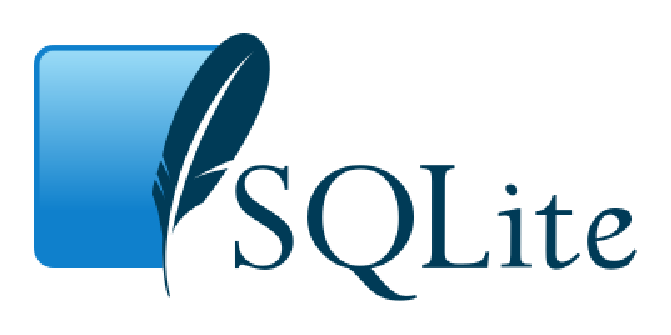
\includegraphics[scale=0.3]{design/figs/SQLite370.eps}}
	\caption{SQLite Logo}
	\label{fig:SQLite-logo}
\end{figure}

SQLite is a relational database and provides simple bindings to use in Python\cite{owens-sqlite}.
It implements SQL and is ACID-compliant\cite{haerder-ACID}.
SQLite saves its database to a single file on disk and provides local storage.
It does not use the typical client-server architecture seen in most other database systems
and the code is directly linked in the program itself.
A separated process is not used to run SQLite.

Tribler uses SQLite to persist its data to disk.
Because Tribler already provides integration and uses SQLite,
SQLite was chosen to be used to persist the blocks.
SQLite adequately meets the design goals needed for the persistence layer of MultiChain.

The data in the SQLite database is readily available.
Queries can be executed directly.
Because there is not another process or server that needs to be contacted latency is reduced.
Concurrency is handled by the SQLite library.

Information stored in a SQLite database is inserted and retrieved using SQL\cite{date-sql}.
SQL allows easy information retrieval and can be used to retrieve specific information.
Using SQL information can easily be retrieved necessary to verify the chain.

ACID-compliance guarantees that transactions are comitted reliably.
The database is stored locally on hard disk.
This is done in a single file and has no redudant backups.
The operator of the node will be responsible to make redudant backups,
but this is trivial for a single file.
The file can be used by any SQLite library on any computer.

\subsection{Persistence layer}
A persistence layer is added to the MultiChain community
that provides all functionality to persist blocks and query blocks.
This layer extends and uses functionality of the Database class in Dispersy.
An overview of the layering in the software architecture can be seen in Figure \ref{fig:persistence-layer}.

\begin{figure}
	\centerline{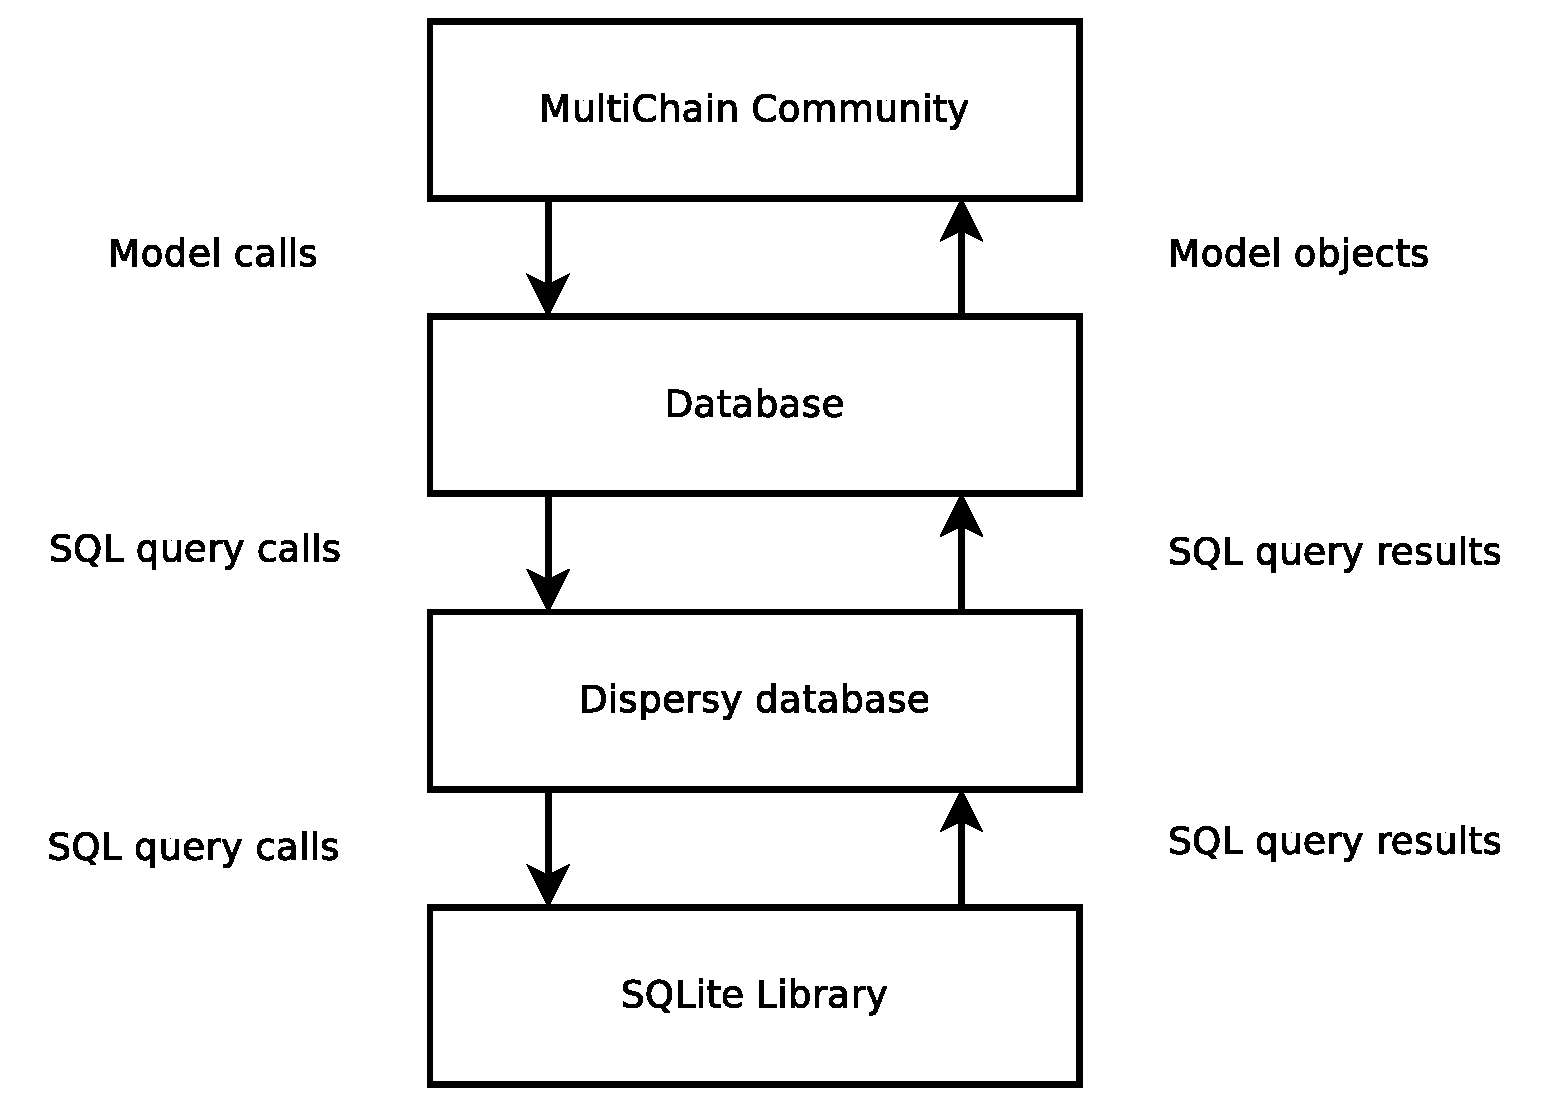
\includegraphics[scale=0.3]{design/figs/persistence-layer.eps}}
	\caption{Persistence layering in the software architecture}
	\label{fig:persistence-layer}
\end{figure}

The MultiChain Community calls functions in the persistence layer that have implicit knowledge about the model.
The Persistence layer formats SQL queries and passes these to the Dispersy layer.
The Dispersy layer performs some sanitation checks and passes these queries to the SQLite Library.
The SQL Library and Dispersy layer returns the result of the SQL query.
These results are transformed by the Persistence layer into objects from the Model usable by the MultiChain Community.

The only information that is present are blocks.
The information all fit within one table.
A single block is saved as a single record called a row in a relation database.
Every attribute of a block is a single column in the row.
An overview of every attribute and the size of the attribute can be seen in Table \ref{table:block_size}.
This makes every attribute queryable in the database.
This was chosen to be extentible and usable when the next incremental steps are implemented.
It is presently unknown precisly what information will be needed,
so every information is now made available for the future.

\subsection{Dispersy database}
Dispersy is an elastic database and keeps track of information on its own.
A record is kept of any message that can be retrieved using a message id.
The message is saved in a converted format and will be decoded when the message is retrieved.

Instead of storing information in a separate database,
the information could have been retrieved from the Dispersy database.
But the Dispersy database is not queryable.
All the information is stored in a converted format
that prevents queries to search the message for its contents.
For this reason, the dispersy database is not used and a separate database is used.







